\documentclass[a4paper,11pt]{refart}

\usepackage[utf8]{inputenc}
\usepackage[T1]{fontenc}

\usepackage{textcomp}
\usepackage[lining,tabular]{fbb}

\usepackage{microtype}

\usepackage{graphicx}
\usepackage{enumitem}
\setlist{leftmargin=*}
\usepackage{listings}
\lstset{basicstyle=\ttfamily,frame=single,xleftmargin=3em,xrightmargin=3em}
\usepackage[os=win]{menukeys}
\renewmenumacro{\keys}[+]{shadowedroundedkeys}
\usepackage{framed}
\usepackage{etoolbox}
\AtBeginEnvironment{leftbar}{\sffamily\small}

\usetikzlibrary{chains,arrows,shapes,positioning}
\usepackage{hyperref}

\renewcommand\abstractname{Resumen}
\renewcommand{\contentsname}{Tabla de contenido}

\title{Lab. 03: Pre-procesamiento de señales sísmicas}
\author{David Duran (\url{davidamos.duran@unmsm.edu.pe})\\\url{https://totallynotdavid.github.io/}}
\date{\url{https://github.com/totallynotdavid/Teleseismic_Body-Wave_Inversion/}\\Versión 1.0 - 14 de noviembre, 2023}
\begin{document}
\maketitle

\begin{abstract}
    Este laboratorio ofrece un método automatizado para descargar, convertir y preparar datos sísmicos, enfocándose en ondas de cuerpo telesísmicas. Detalla el uso de un script en Python para obtener datos en formato miniSEED y metadatos en XML, y su conversión a formatos SEED (dataless SEED) y SAC mediante la herramienta rdseed. El objetivo es optimizar la eficiencia y estandarizar la gestión de datos sísmicos.
\end{abstract}

\tableofcontents
\clearpage

\section*{Flujo de trabajo del script}

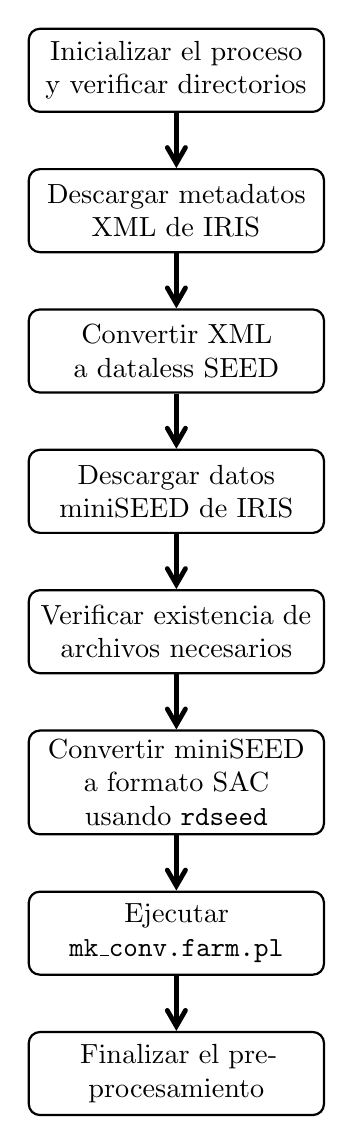
\begin{tikzpicture}
  \tikzset{
    every node/.style={
      on chain,
      draw,
      thick,
      rounded corners,
      minimum height=3em,
      text width=10em,
      align=center
    },
    line/.style={
      draw,
      thick,
      -latex',
      shorten >=2pt
    },
    every join/.style={line}
  }
  
  \begin{scope}[start chain=going below, node distance=0.7cm]
  \node (init) {Inicializar el proceso y verificar directorios};
  \node (downmeta) {Descargar metadatos XML de IRIS};
  \node (convertmeta) {Convertir XML a dataless SEED};
  \node (downseed) {Descargar datos miniSEED de IRIS};
  \node (convseed) {Verificar existencia de archivos necesarios};
  \node (seedtosac) {Convertir miniSEED a formato SAC usando \texttt{rdseed}};
  \node (postprocess) {Ejecutar \texttt{mk\_conv.farm.pl}};
  \node (end) {Finalizar el pre-procesamiento};
  \end{scope}

  \path[draw,line width=0.4ex, ->,>= angle 60]
  (init) edge (downmeta)
  (downmeta) edge (convertmeta)
  (convertmeta) edge (downseed)
  (downseed) edge (convseed)
  (convseed) edge (seedtosac)
  (seedtosac) edge (postprocess)
  (postprocess) edge (end);

\end{tikzpicture}

\section{Introducción}

Este documento sirve como una guía detallada para la automatización en la adquisición y procesamiento de datos sísmicos, con aplicaciones específicas en el modelo de Kikuchi y Kanamori. 
Aborda cómo este proyecto mejora la recolección y preparación de datos geofísicos y su importancia en el contexto más amplio de la investigación sísmica. 
Este trabajo es parte del proyecto de tesis ``Aspectos físicos de la fuente del terremoto de Yauca-Arequipa de 2013 (7.1 Mw)'' por David Duran, supervisado por el Dr. Cesar Jimenez. 
Se incluyen ejemplos prácticos y enlaces a recursos adicionales para comprender mejor las herramientas utilizadas.

\section{Instalar dependencias}

\subsection{Prerrequisitos}

Antes de comenzar la instalación, asegúrate de que tu sistema cumpla con los siguientes prerrequisitos:

\begin{itemize}
  \item Sistema operativo: Ubuntu 20.04 LTS o superior.
  \item Memoria: Al menos 4 GB de RAM.
  \item Espacio en disco: 10 GB de espacio libre.
  \item Conexión a Internet para descargar las dependencias.
\end{itemize}

\subsection{Herramientas necesarias}

\begin{leftbar}
  El proceso de instalación de las siguientes herramientas puede variar según el sistema operativo. Para usuarios de Ubuntu (GNU Linux), hemos facilitado este proceso con el script \texttt{dependencies.sh}. Encuentra detalles adicionales en el archivo \texttt{README.md} en nuestro repositorio de GitHub. Para problemas durante la instalación, consulta las secciones de 'Preguntas frecuentes' o 'Solución de problemas' en los sitios web de las herramientas.
\end{leftbar}

La instalación de herramientas esenciales es el primer paso para asegurar un flujo de trabajo eficiente en el análisis sísmico. Por esto, es necesario instalar una serie de dependencias:

\begin{itemize}
  \item \textbf{rdseed}: Es utilizado para leer e interpretar archivos en formato SEED, el estándar de la Federación de Redes Sismográficas Digitales (FDSN, por sus siglas en inglés) para datos sísmicos. En nuestro proyecto, rdseed es utilizado para convertir datos descargados en formato miniSEED a SAC. En 2018 dejó de recibir soporte, sin embargo puedes descargar rdseed desde: \url{http://www.iris.edu/pub/programs/rdseedv5.3.1.tar.gz} o compilarlo desde el código fuente en: \url{https://github.com/iris-edu-legacy/rdseed}.

  \item \textbf{stationxml-seed-converter}: Es utilizado para convertir metadatos sísmicos entre los formatos dataless SEED y FDSN-StationXML. En nuestro proyecto, usamos esta herramienta para transformar metadatos descargados en formato XML a dataless SEED, lo que permite su posterior procesamiento con rdseed. Esta herramienta es un programa de línea de comandos escrito en Java, por lo que es importante tener Java instalado en el sistema. Descarga el conversor desde: \url{https://github.com/iris-edu/stationxml-seed-converter}.

  \item \textbf{Java}: Importante para ejecutar el `stationxml-seed-converter`. En sistemas basados en Ubuntu, instala Java con el comando: \texttt{sudo apt install default-jre}.

  \item \textbf{Seismic Analysis Code (SAC)}: Este software se utiliza para el análisis detallado de eventos sísmicos. En nuestro proyecto, SAC es importante para operaciones posteriores de análisis y procesamiento de los datos sísmicos convertidos por rdseed. SAC no está disponible públicamente, pero puedes solicitarlo en: \url{http://ds.iris.edu/ds/nodes/dmc/forms/sac/}.

  \item \textbf{Perl}: Un lenguaje de programación utilizado para ejecutar scripts que manejan archivos de datos sísmicos. Aunque no se usa directamente en nuestro script principal, Perl es útil para tareas de automatización y procesamiento de datos relacionados, como los proporcionados por algunas herramientas de rdseed y SAC. Instala Perl en Ubuntu con: \texttt{sudo apt install perl}.
\end{itemize}

\subsubsection{Pasos para la instalación}

Sigue estos pasos para preparar tu entorno de trabajo:

\begin{enumerate}
  \item Clona el repositorio con las dependencias y scripts:
  \begin{verbatim}
  git clone https://github.com/totallynotdavid/Teleseismic_Body-Wave_Inversion/
  \end{verbatim}

  \item Navega al directorio del repositorio:
  \begin{verbatim}
  cd Teleseismic_Body-Wave_Inversion
  \end{verbatim}

  \item Asigna permisos de ejecución al script \texttt{dependencies.sh}:
  \begin{verbatim}
  chmod +x ./scripts/bash/dependencies.sh
  \end{verbatim}

  \item Ejecuta \texttt{dependencies.sh} para instalar las dependencias. Consulta \texttt{INSTALL.md} en caso de errores:
  \begin{verbatim}
  ./scripts/bash/dependencies.sh
  \end{verbatim}
\end{enumerate}

\section{Pre-procesamiento}

\subsection{Preparación de datos}

Antes de utilizar el modelo de Kikuchi y Kanamori, necesitas preparar tus datos en el formato SAC \footnote{SAC headers contienen información sobre la inclinación y el azimut.}. Para ello, utiliza el siguiente script de Python, el cual automatiza la descarga y el procesamiento inicial de los datos sismicos.

\begin{enumerate}
\item Ejecuta el script con Python:
\begin{verbatim}
python3 /scripts/python/fetch_and_process.py
\end{verbatim}
El script procederá con la descarga y conversión de datos, preparándolos para el análisis con el modelo.
\item Para eliminar archivos innecesarios y mantener el orden, utiliza el script de limpieza proporcionado:
\begin{verbatim}
chmod +x /scripts/bash/cleaning.sh
./scripts/bash/cleaning.sh
\end{verbatim}

\end{enumerate}

\subsection{Procesamiento final con Perl}

Finalmente, para convertir los datos al formato deseado por el modelo:
  \begin{enumerate}
  \item Navega a la carpeta de scripts de Perl y copia el script necesario a la carpeta de datos:
  \begin{verbatim}
  cp mk_conv.farm.pl /data/preprocesamiento/
  cd /data/preprocesamiento/
  \end{verbatim}
  \item Ejecuta el script de Perl para completar la conversión:
  \begin{verbatim}
  perl mk_conv.farm.pl
  \end{verbatim}
\end{enumerate}
Con estos pasos, tendrás los datos listos para ser utilizados en el pipeline del modelo de Kikuchi y Kanamori.

\section{Detalles técnicos}

El proceso de procesamiento de señales sísmicas se apoya en una serie de scripts diseñados para automatizar las tareas que van desde la adquisición de los datos hasta su preparación definitiva para el análisis correspondiente con el modelo. A continuación, se delinean los componentes técnicos fundamentales de la fase inicial del flujo de trabajo, establecido por el autor. Esta fase se maneja de forma independiente al modelo de Kikuchi y Kanamori.

De forma general, el script hace lo siguiente:

\begin{enumerate}
  \item Define las estaciones sísmicas y los rangos de tiempo de interés.
  \item Realiza solicitudes HTTP para descargar datos sísmicos en formato miniSEED y metadatos en formato XML utilizando las APIs brindadas por IRIS.
  \item Convierte los metadatos XML a formato dataless SEED utilizando herramientas Java.
  \item Prepara los archivos miniSEED para su procesamiento posterior.
\end{enumerate}

\subsection{Descarga de datos}

Para la automatización de los requests con la base de datos de SAGE (\textit{Seismological Facility for the Advancement of Geoscience}), se ha desarrollado el script \texttt{fetch\_and\_process.py}. Este script está concebido para facilitar la recolección eficiente de los datos sísmicos junto con sus respectivos metadatos. Es necesario, claro está, definir las estaciones apropiadas y los rangos de tiempo apropiados para el investigador.

En el pasado, la adquisición de archivos en formato SAC se realizaba automáticamente a través del portal Wilber 3; sin embargo, dicha funcionalidad fue descontinuada en el 2021 en favor de los archivos miniSEED. A raíz de esto, es ahora requisito construir el archivo SAC manualmente, utilizando los datos obtenidos en formato miniSEED, complementándolos con los metadatos en el formato dataless y los polos y ceros necesarios.

\begin{itemize}
    \item \textbf{Metadatos:} El servicio web FDSN se emplea para obtener metadatos en formato XML, que ofrecen información detallada sobre las estaciones sísmicas, incluyendo sus ubicaciones, equipamiento y características de las señales registradas. Estos metadatos son cruciales para la interpretación correcta de los datos sísmicos.
    \item \textbf{Datos Sísmicos:} Se descargan los registros sísmicos en formato miniSEED. Este formato es la elección estándar en la industria para el almacenamiento y transmisión de datos sísmicos debido a su eficiencia y amplia adopción, lo que asegura compatibilidad y facilidad de uso en diversas aplicaciones de análisis.
\end{itemize}

El script está configurado para procesar datos de múltiples estaciones sísmicas.

\subsection{Verificación de archivos necesarios}

Antes de proceder con la conversión de miniSEED a SAC, el script realiza una verificación para asegurarse de que todos los archivos necesarios estén presentes. Esto incluye la presencia de los archivos dataless y los archivos miniSEED. Si falta algún archivo, el script alertará al usuario y detendrá el proceso para evitar errores en el procesamiento posterior.

\subsection{Uso de \texttt{rdseed}}

Para la conversión de miniSEED a SAC, se emplea el programa \texttt{rdseed}. Es una herramienta que permite la extracción de datos de archivos SEED (incluyendo miniSEED y dataless SEED) y su conversión a otros formatos, en este caso, al formato SAC utilizado ampliamente en el análisis sísmico.

\subsection{Scripts Perl para procesamiento final}

\texttt{mk\_conv.farm.pl} (brindado por Kikuchi y Kanamori en el manual de su modelo) es utilizado en la etapa final del pre-procesamiento para automatizar el procesamiento de grandes conjuntos de datos. Este script generará dos archivos: \texttt{response} y \texttt{i\_conv.farm}.

\subsection{Entorno de ejecución}

El entorno de ejecución para los scripts está configurado para ser lo más automatizado posible, reduciendo la necesidad de intervención manual y permitiendo que los investigadores se centren en el análisis de los datos en lugar de en su preparación.

\begin{itemize}
\item Se asume que las dependencias y el entorno (Fortran77, Java, Perl) han sido instalados y configurados adecuadamente, según se describe en las secciones previas de la guía.
\item Se espera que el sistema operativo sea compatible con los scripts de Bash y Python, así como con las herramientas Fortran y Perl.
\end{itemize}

\subsection{Documentación y soporte}

El código de cada script está ampliamente documentado internamente para facilitar la comprensión de su funcionamiento y la personalización de los procesos. Para problemas complejos o consultas específicas, se recomienda contactar al autor del script. El correo se encuentra en la portada de este documento.

\bibliographystyle{plain}
\bibliography{refs}
\end{document}